\chapter{Power flow in electromagnetic wave.}
Up till now we have seen that a time varying electric and magnetic field constitute a wave phenomenon. Thus this wave requires some power or energy to flow with. In this lecture we look at the power flow associated with electromagnetic waves. We do some derivation starting with the Maxwell?s Equation and find out the power flow associated with a time varying electromagnetic field.\\

Up till now, we have investigated a wave which is called uniform plane wave i.e. a wave propagation in an unbound medium. However, in developing the power flow equations associated with electromagnetic waves, we would do a general analysis and not restrict our focus to uniform plane waves, at the end we find out the power flow associated with uniform plane waves which we have discussed in lectures 25 and 26. So whenever we have the beginning of analysis in electromechanics, we basically go back to the Maxwell?s Equations and find answers that are consistent with Maxwell?s equation. Same thing we do have if we are asked a question, we go back to the Maxwell?s Equations. What power do we get for power flow associated with the electromagnetic fields? From Maxwell?s Equation we have;
\begin{align}
\nabla\times\overline{E}=-\frac{\partial\overline{B}}{\partial t} \cdot \end{align} If the permeability of the system is not a function of time,
\begin{align}
\={B}=\mu\={H}\\
\frac{\delta\overline{B}}{\partial t}= -\mu\frac{\delta\overline{H}}{\delta t} =  - \mu\frac{\delta\overline{H}}{\delta t}
\end{align}
 Therefore;\\
\begin{align}
\nabla\times\overline{E} = -\mu \frac{\delta\overline{H}}{\delta t} \end{align} and \begin{align}
\nabla\times\overline{H} =\overline{J} + \frac{\delta\overline{D}}{\delta t}  =  J + \epsilon\frac{\delta\overline{E}}{\delta t} 
\end{align}
if permeability  $(\epsilon) $ is not a function of time.\\
We start with these two basic equations and then try to investigate the power flow associated with electric and magnetic fields. We essentially make use of the vector identities and then try to find out the meaning to some expressions we would get from using the vector identities.\\

\begin{align}\nabla \cdot ( \overline{A}\times\overline{C} ) = C \cdot (\nabla\times\overline{A}) - \overline{A}\cdot(\nabla\times\overline{C}) \end{align} For arbitrary vectors $\overline{A}$ and $\overline{C}$,\\\\ Let $\overline{A}$ be the electric field $\overline{E}$and $ \overline{C} $ be the Magnetic Field $\overline{H}$, substituting for $\overline{A}$ as $\overline{E}$ and $\overline{C}$ as $\overline{H}$ into equation (5.4), we have;\begin{align}
\nabla\cdot(\overline{E}\times\overline{H})= \overline{H}\cdot(\nabla\times\overline{E})-\overline{E}\cdot(\nabla\times\overline{H})\end{align} Now Substituting for $\nabla\times\overline{E}$ and $\nabla\times\overline{H}$, we have;
\begin{align} \nabla\cdot(\overline{E}\times\overline{H})=
\overline{H}\cdot(-\mu\frac{\delta\overline{H}}{\delta t}) - \overline{E}\cdot(\overline{J}+\epsilon\frac{\delta\overline{E}}{\delta t})
\end{align}\\ Recall from vector identities, we  have that;\\ $\frac{\delta}{\delta t}(\overline{A}\cdot\overline{C})= \overline{A}\cdot\frac{\delta\overline{C}}{\delta t}+\overline{C}\cdot\frac{\delta\overline{A}}{\delta t}$ \\
$\frac{\delta}{\delta t}(\overline{A}\cdot\overline{A})= \overline{A}\cdot\frac{\delta\overline{A}}{\delta t}+\overline{A}\cdot\frac{\delta\overline{A}}{\delta t} = 2\overline{A}\cdot\frac{\delta A}{\delta t}$
\\\\
Making $\overline{A}\frac{\delta A}{\delta t} $ the subject of formula,\\we have;\\ \begin{align}
\overline{A}\cdot\frac{\delta\overline{A}}{\delta t}=\frac{1}{2}\frac{\delta}{\delta t}(\overline{A}\cdot\overline{A})=\frac{1}{2}\frac{\delta}{\delta t} |A|^{2} \end{align}
having refreshed ourselves with these identities, we can deduce from equation (27.9)  that;\begin{align}
\nabla\cdot(\overline{E}\times\overline{H})=	-\mu(\overline{H}\cdot\frac{\delta\overline{H}}{\delta t})-\overline{E}\cdot\overline{J}-\epsilon(\overline{E}\cdot\frac{\delta\overline{E}}{\delta t})\end{align}
therefore, relating equation (27.11) to equation (27.10) we have;
\begin{align}
\nabla\cdot(\overline{E}\times\overline{H})=-\frac{\mu}{2}\frac{\delta}{\delta t}|\overline{H}|^{2} -  \frac{\epsilon}{2}\frac{\delta}{\delta t}|\overline{E}|^{2}-\overline{E}\cdot\overline{J} \end{align}
We can investigate this expression over a closed surface or volume to have some meaning associated with these quantities.\\\\
\begin{align*}
\iiint_{v}\nabla\cdot(\overline{E}\times\overline{H})dv  = \iiint_v-\frac{\mu}{2}\frac{\delta}{\delta t}|\overline{H}|^{2}dv-\\ \iiint_{v}\frac{\epsilon}{2}\frac{\delta}{\delta t}|\overline{E}|^{2}dv -\iiint_{v}\overline{E}\cdot\overline{J}dv 
\end{align*}\\\\
If we assume that volume enclosed is not varying as a function of time i.e. fixed volume, that is to say that  the field varies with time but space does not vary with time. We can take $\frac{\delta}{\delta t}$ out of the equation and apply divergence theorem on $ \int_{v}\nabla_{e}(\overline{E}\times\overline{H}) $ to change it to a closed surface integral.\\\\
\begin{math}
\iint(\overline{E}\times\overline{H})\cdot\overline{d}a  =  -\frac{\delta}{\delta t}  \iiint_{v}\frac{\mu}{2}|\overline{H}|^{2}dv -  \frac{\delta}{\delta t}\iiint_{v}\frac{\epsilon}{2}|\overline{E}|^{2}dv  -  \iiint_{v}\overline{E}\cdot\overline{J}dv 
\end{math}\\
we now substitute $ \overline{J}=\sigma\overline{E}, $ into equation (27.12) to get; \\\\
$\overline{E}\cdot\overline{J}=\overline{E}\sigma\overline{E}=\sigma\overline{E}\overline{E}=\sigma|\overline{E}|^{2} $\\\\
$ \oint(\overline{E}\times\overline{H})\overline{d}a $ = - $ \frac{\delta}{\delta t}\int_{v} \frac{\mu}{2}|\overline{H}|^{2}dv$ - $ \frac{\delta}{\delta t}\int_{v}\frac{\epsilon}{2}|\overline{E}|^{2}dv$\\
-$ \int_{v}\sigma|\overline{E}|^{2}dv $
\\
\\
where;
\\
$ \iiint_{v}\frac{\mu}{2}|\overline{H}|^{2}dv $ (\begin{small}
Tells us the total Magnetic energy stored in that volume V
\end{small})\\
and\\
$ \iiint_{v} \frac{\epsilon}{2}|\overline{E}|^{2}dv $ (\begin{small}
	Tells us the total electric energy stored in that volume V     
\end{small})\\
-$\frac{\delta}{\delta t}\iiint_{v}\frac{\mu}{2}|\overline{H}|^{2}dv$
(\begin{small}
	Shows us the rate of change of Magnetic (decrease) energy stored                            in a volume v i.e. decrease in energy over time     
\end{small})\\
-$\frac{\delta}{\delta t}\int_{v}\frac{\epsilon}{2}|\overline{E}|^{2}dv$
(\begin{small}
	Shows the rate of change of Electric (decrease) energy stored                            in a volume v i.e. decrease in energy as a function of time    
\end{small})\\ 
-$\int_{v}\sigma|\overline{E}|^{2}dv$
(\begin{small}
	Shows the Ohmic loss in that volume or power loss in the volume because of finite conductivity in the medium.   
\end{small})\\ \\
So if we have a total energy enclosed in a surface, these 3 total losses combine must be equal to the outward energy going out from the closed surface (s), Since there is no other mechanism for energy consumption. From law of conservation of energy, we get that $ \oint(\overline{E}\times\overline{H})\overline{d}a $ must represent the flow of energy coming out from the closed surface. So $ \oint(\overline{E}\times\overline{H})\overline{d}a $ (the net power outflow from a closed surface)  gives the net power flow of the electric and magnetic field from that closed surface. This is called \textbf{ POYNTING THEOREM}.\footnote{John Henry Poynting (Born 9, September 1852 and died 30, March 1914. He was an English physicist. He was a professor of physics at Mason Science College, from 1880 to 1900, and then the successor institution, the University of Birmingham until his death.\\ 
	He is Known For:Poynting vector, Poynting Effect, Poynting's Theorem \\
	Poynting was the youngest son of Thomas Elford Poynting, a Unitarian minister}
The poynting theorem states that the cross product of electric and magnetic field integrated over a closed surface gives the total power flow from the closed surface. Now we have seen the quantity which represents the total power flow, then 
$\overline{E}\times\overline{H}$ is essentially the power density on the surface. So that when this power density is integrated over an area, it gives the total power flow from the surface.	 It should be kept in mind that as the total power flow gives the net power flow, $\overline{E}\times\overline{H}$ Should give the power density at any point on the surface of the sphere is arbitrary definition.  The theorem does not state that $\overline{E}\times\overline{H}$ represent the power density or power flow per unit area at every point on the surface of the volume. What it is telling us is that the total power coming out of a close surface is $\oint_{s}(\overline{E}\times\overline{H})$. So saying that $\overline{E}\times\overline{H}$ is the power density which is true for every point on the surface of a SPHERE (Because of Symmetry). It is arbitrary we take power density from here. It so happens that most of the time in practice, this arbitrary definition gives the power density correctly. However, it should be said that if knowing $\overline{E}\times\overline{H}$ , one already knows power density  at every point on the surface of this volume. This statement is not correct. In fact there are many special cases where $\overline{E}\times\overline{H}$  may give power flow where in actual fact there is no power flow at that point. So while using $\overline{E}\times\overline{H}$  as power density, one should be very careful. In most practical situations however, the arbitrary definition that $\overline{E}\times\overline{H}$  gives power density at any location normally is valid.


So we have an important quantity called a power flow density $ \overline{P}=\overline{E}\times\overline{H} $ where $  \overline{P}  $ is called a POYNTING VECTOR for these fields. Poynting vector is an important concept in electromagnetic wave as it tells the power flow associated with any particular point in space and also tells in which direction the power is flowing.The first thing we note here is that if you have electric and magnetic field, the poynting vector is the direction perpendicular to both $ \overline{E} $ and  $ \overline{H} $. So if $  \overline{P}  $  has to be non zero in terms of power flow, then $ \overline{E} $ and  $ \overline{H} $ should not be parallel to each other. In a case where  $ \overline{E} $ and  $ \overline{H} $ are parallel to each other, then  $ \overline{E}\times\overline{H} $=0 and this connotes that there will be no net power flow associated with this. So only when the component of electric and magnetic field  are perpendicular to each other would they contribute to power flow and the direction of power flow is perpendicular to $ \overline{E} $ and  $ \overline{H} $    fields. It should be noted that for we to have a power flow $ \overline{E} $ and  $ \overline{H} $  must cross each other, whenever $ \overline{E} $ and  $ \overline{H} $ Crosses each other, there is a possibility of power flow. We use the word possibility here because this quantity   $ \overline{E}\times\overline{H} $ is telling you the so called instantaneous power if we know the value of ?. and  $ \overline{E} $ and  $ \overline{H} $. At that instant of time at some point in space,we can always find out $ \overline{E}\times\overline{H} $. At that instant of time, we get $  \overline{P}  $ which will give the poynting vector at that instance of time. It is possible that even if $  \overline{P}  $ is finite at some instance of time, there may be  a net power flow over long time periods. That is in time average sense, there may not be power flow associated with that system. So Poynting Vector $  \overline{P}  $ which we defined as $ \overline{E}\times\overline{H} $  serves the the purpose of defining the power flow. But in Practical System, a more useful quantity would be the time average value of the Poynting Vector, because the poynting vector at some instant of time may be negative and that is like getting negative power. Of course when dealing with space, we can say negative power flow means direction change. All these complications come in simply if we use $ \overline{E}\times\overline{H} $ to get  $  \overline{P}  $. since $  \overline{P}  $  can be positive or negative and $  \overline{P}  $  can be a complex quantity too if there is a phase difference between $ \overline{E} $ and  $ \overline{H} $ with time. So what we do is, we try to get the time average value of the poynting vector and it is a much more useful quantity for finding out if there is a net flow of power associated with the Electric and Magnetic fields. \\

As we have seen earlier, we are interested only in analysis of time harmonic fields, so we assume that electric and magnetic fields are varying sinusoidally as a function of time. The only thing being a phase difference between $ \overline{E} $ and  $ \overline{H} $ , we are then asked what is the average power flow associated with $ \overline{E} $ and  $ \overline{H} $ In this case.\\


Now we define the general time varying electric and magnetic fields which varies as a function of space and time as;\\
\\
$ \overline{E}=\overline{E_{o}} e^{jwt+j\phi_{e}}$ ,\\
$ \overline{H}=\overline{H_{o}} e^{jwt+j\phi_{h}}$\\
We take the unit vector associated with $ \overline{E_{o}} $ and  $ \overline{H_{o}} $ as $ \hat{e} $ And $ \hat{h} $, so we remember that we are only taking either the real of imaginary part of $ e^{jwt} $ for simple analysis. It doesn?t mean $ \overline{E} $ cannot be complex. But for simplicity,\\
$ \overline{E}=R_{e}(E_{o}e^{jwt}e^{j\phi e} )\cdot\hat{e} $   \\
$ \overline{H}=R_{e}(H_{o}e^{jwt}e^{j\phi h} )\cdot\hat{h} $ \\
where  $ \hat{e} $ and $ \hat{h} $ 
gives the unit vector of the electric and magnetic field, $ \phi_{e} $ and $ \phi_{h} $ are the phase electric and magnetic field and $ E_{o} $ and  $ H_{o} $ are the amplitude of electric  and magnetic fields. So the real parts give instantaneous value of electric and magnetic field. Once this is known, we can find the poynting vector at that instant of time.
$ \overline{E}(t)=E_{o}\cos(\omega t+\phi_{e})\hat{e} $ \\
$ \overline{H}(t)=H_{o}\cos(\omega t+\phi_{h})\hat{h} $\\
The power flow density at that instant t, is the poynting vector  $ \overline{P} $  would be ;\\\\
$ \overline{P}=\overline{E}\times\overline{H} $ = $ E_{o}H_{o}\cos(\omega t+\phi_{e}) \cos(\omega t+\phi_{h}) (\hat{e}\times\hat{h})$ = $ \frac{ E {o}H {o}}{2} (\cos(\phi_{e}-\phi_{h})+\cos(2\omega t + \phi_{e}+\phi_{h}))  (\hat{e}\times\hat{h})$ 
\\\\
		How did we get to the last expression, we will see below.
		From compound angle formulas, we have\\\\
		$ \cos(\omega t+\omega t) =\cos\omega t\cos\omega t-\sin\omega t\sin\omega t =\cos^{2}\omega t-\sin^{2}\omega t=\cos^{2}\omega t-(1-\cos^{2}\omega t)$\\\\
		simplifying further,we get\\\\
		$ 2\cos^{2}\omega t-1 $ or $ \cos^{2}\omega t=\frac{\cos^{2}\omega t+1}{2} $ ;\\
		$ \sin(\omega t+\omega t) =\sin\omega t\cos\omega t-\cos\omega t\sin\omega t$ =
		simplifying further,we get\\
		$ 2\sin\omega t\cos\omega t$ or $  \sin\omega t\cos\omega t = \frac{\sin2\omega t}{2} \\
		$\\
$\overline{P}= \overline{E}\times\overline{H}=E_{o}H_{o}\cos(\omega t+\phi_{e})\cos(\omega t+\phi_{h})\hat{e}\times\hat{h} $\\
=$ E_{o}H_{o}[(\cos\omega t\cos\phi_{e}-\sin\omega t\sin\phi_{e})(\cos\omega t\cos\phi_{h}-\sin\omega t\sin\phi_{h})]\hat{e}\times\hat{h} $\\
= $ E_{o}H_{o}[\cos^{2}\omega t\cos\phi_{e}\cos_{h}-\cos\omega t\sin\omega t\cos\phi_{e}\sin\phi_{h}-\cos\omega t\sin\omega t\sin\phi_{e}\cos\phi_{h}+\sin^{2}\omega t\sin\phi_{e}\sin_{h}]\hat{e}\times\hat{h}$\\
=$E_{o}H_{o}[\cos^{2}\omega t\cos\phi_{e}\cos\phi_{h}+ ( 1 - \cos^{2}\omega t)\sin\phi_{e}\sin\phi_{h} -\cos\omega t\sin\omega t(cos\phi_{e}\sin\phi_{h} +\sin \phi_{e}\sin\phi_{h})]\hat{e}\times\hat{h} $\\\\
=$E_{o}H_{o}[\cos^{2}\omega t(\cos\phi_{e}\cos\phi_{h}-\sin\phi_{e}\sin\phi_{h})+\sin\phi_{e}\sin\phi_{h}-\cos\omega t\sin\omega t()\cos\phi_{e}\sin\phi_{h}+\sin\phi_{e}\cos\phi_{h}] \hat{e}\times\hat{h} $\\\\=   $ E_{o}H_{o}[\cos^{2}\omega t\cos(\phi_{e}+\phi_{h})+\sin\phi_{e}\sin\phi_{h}-\cos\omega t\sin\omega t\sin(\phi_{e}+\phi_{h})      ]\hat{e}\times\hat{h} $ \\\\
=$E_{o}H_{o} [(\frac{\cos\omega t+1}{2})\cos(\phi_{e}+\phi_{h})+\sin\phi_{e}\sin\phi_{h}-\frac{\sin2\omega t}{2}\sin(\phi_{e}+\phi_{h})] \hat{e}\times\hat{h}  $\\\\
=$E_{o}H_{o}[\cos2\omega t\cos(\phi_{e}+\phi_{h})-\sin2\omega t\sin(\phi_{e}+\phi_{h})+\frac{1}{2}\cos(\phi_{e}+\phi_{h})+\sin\phi_{e}\sin\phi_{h}]\hat{e}\times\hat{h} $\\\\$  =E_{o}H_{o}[\frac{1}{2}\cos(2\omega t+\phi_{e}+\phi_{h})+\frac{1}{2}\cos(\phi_{e}+\phi_{h})+\sin\phi_{e}\sin\phi_{h}]\hat{e}\times\hat{h} $\\\\ =$E_{o}H_{o}[\frac{1}{2}\cos(2\omega t+\phi_{e}+\phi_{h})+\frac{1}{2}\cos\phi_{e}\cos_{h} -\frac{1}{2}\sin\phi_{e}\sin\phi_{h}+\sin\phi_{e}\sin\phi_{h}]\hat{e}\times\hat{h} $\\\\$  E_{o}H_{o}[\frac{1}{2}\cos(2\omega t+\phi_{e}+\phi_{h})+\frac{1}{2}\cos\phi_{e}\cos_{h} +\frac{1}{2}\sin\phi_{e}\sin\phi_{h}]\hat{e}\times\hat{h} $\\\\$=\frac{ E_{o}H_{o}}{2}[\cos(\phi_{e}-\phi_{h})+\cos(2\omega t+\phi_{e}+\phi_{h})]\hat{e}\times\hat{h} $\\\\
So when we take average of this over the period of the signal then $\cos(2\omega t+\phi_{e}+\phi_{h})$ will go to zero. Positive area cancels negative area. It corresponds to a wave form having 2f as its frequency. So over a period corresponding to $ T=\frac{2\pi}{\omega} $ the time average $ \overline{P}_{av} $ is; $ \frac{1}{T}\int^{T}_{0}\overline{P}dt $ with $ T=\frac{2\pi}{\omega} $.\\\\$\overline{P}_{av}=\frac{1}{T}\int^{T}_{0} \frac{ E_{o}H_{o}}{2} \cos(\phi_{e}-\phi_{h})dt$ $( \hat{e}\times\hat{h}) $ \\\\
$ \frac{E_{o}H_{o}}{2} \cos(\phi_{e}-\phi_{h})(\hat{e}\times\hat{h}) $\\\\
=$\frac{1}{2} R_{e}[(E_{o}e^{j\omega t+j\phi_{e}}+\hat{e})\times(H_{o}e^{j\omega t+j\phi_{h}}+\hat{h})] ^{*}  $\\\begin{flushright}
	\begin{small}
		the * above is the conjugate.
	\end{small}
\end{flushright} But Originally;\\\\
$ \overline{E}=\overline{E_{o}}e^{j\omega t+j\phi_{e}}$\\
and\\\\
$ H=\overline{H_{o}}e^{j\omega t+j\phi_{e}} $\\\\ We now have the average power to be;\\
$\overline{P}_{av}=R_{e}(\overline{E}\times\overline{H}^{*})$\\\\



This means that if we know the electric and magnetic field in complex forms, i.e. the electric and magnetic field may not be in time phase. In general, we can calculate $ \overline{E}\times\overline{H}^{*} $, the real part of that. Taking $ \frac{1}{2} $ of it gives the average power flow which is associated with that electromagnetic wave. So $\overline{P}_{av}=\frac{1}{2}R_{e}(\overline{E}\times\overline{H}^{*})$ is a real quantity. All these problems we had with instantaneous power flow, $ \overline{P}=\overline{E}\times\overline{H} $ complex depending on phase between $ \overline{E} $ and $ \overline{H} $, have now been taken care of. This also tells the overall power flow which is associated with this field at a particular location, the instantaneous poynting vector might be negative or positive. But the average power poynting vector will always be positive and that gives the net power flow associated with those electric and magnetic fields.

This is the concept regularly used in finding out the power flow associated with magnetic waves. Again you have for average power flow that $ \overline{E} $ and $ \overline{H} $ fields are perpendicular (or have components perpendicular to each other), only then would we have a cross product which will be non zero.
Secondly the electric and magnetic field should not be in TIME QUADRATURE. This means the electric and magnetic field should not differ by a phase of $90^{o}$. If this happens, $ R_{e}(\overline{E}\times\overline{H}^{*})=0 $ and then we will not have any real power flow associated with the field at that point. It is generally possible that if you take the electric and magnetic field, you get complex power. The real part of the quantity gives the net power flow at that location and the imaginary part (j conjugate ) gives the power oscillating around a point. At some point, the power is coming back essentially so imaginary part of $ E\times\overline{H}^{*} $ gives the oscillatory power called the REACTIVE POWER. Whereas the real part gives the net power flow or the RESISTIVE POWER flow at the location. So this concept of Poynting vector and the average Poynting vector is  very important because by using this concept, we can calculate the net power flow at a particular location.

We can then apply this concept to a case of uniform plane wave. How much power density does a uniform plane wave carry when it travels in a media? In Uniform plane waves, electric and magnetic fields are perpendicular to each other. With $ \overline{E} $ and $ \overline{H} $ shown below.\\\\\\ \begin{figure}[h]
	\centering
	\textsc{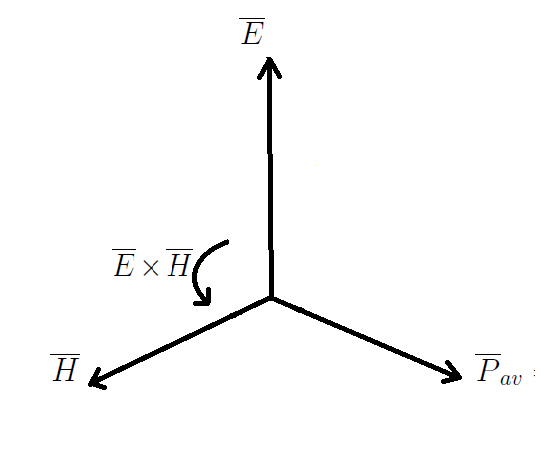
\includegraphics[height=5cm]{../TeX_files/cc}}
	\vspace{-10pt}
	\caption{Direction of power flow of an electromagnetic wave}
\end{figure}\\\\\\\\\\\\\\The direction of power flow is given by the right hand rule. $ \overline{E}\times\overline{H} $ as we realize has the direction of $ \overline{P}_{av} $ which is also the same as the direction of wave propagation. As we have seen in case of uniform plane wave, $ \overline{E} $ , $ \overline{H} $ and direction of propagation are perpendicular to each other.\\If we say the electric field is $ \overline{E}=E_{o}e^{-j\beta z}\hat{x} $ having phase variation of Z therefore;\\\\
 $ \overline{H}=H_{o}e^{-j\beta z}\hat{y} $,\\\\ $ \overline{P}_{av}=\frac{1}{2}R_{e}(\overline{E}\times\overline{H}^{*})\\\overline{P}_{av}=\frac{1}{2}R_{e}(E_{o}e^{-j\beta z}H_{o}e^{+j\beta z}\hat{x}\times\hat{y})\\\overline{P}_{av}=\frac{1}{2}R_{E}(E_{o}H_{o}\hat{z})=\frac{1}{2}(E_{o}H_{o}\hat{z}) $\\\\So for uniform plane wave, the average poynting vector will be half $ E_{o}H_{o} $. in direction $ \hat{z} $ with $ \overline{E} $ in $ \hat{x} $ and $ \overline{H} $ in $ \hat{y} $ direction.
Now we can take specific cases for the uniform plane wave in unbound medium in which the wave is propagating. For a DIELECTRIC MEDIUM, $ \overline{E} $ and $ \overline{H} $ are related by the intrinsic impedance of the medium.\\\\
$ \frac{E}{H}=\eta $= intrinsic impedance.\\\\
 Substituting into \\\\
[$ \overline{P}_{av}=\frac{1}{2}(E_{o}H_{o}z^{*}) $] 
\\and making it in terms of electric field,  we have;\\ $ \overline{P}_{av}=\frac{1}{2}E_{o}(\frac{E_{o}}{\eta})^{*}\hat{z} $ This can also be written as\\$ \overline{P}_{ov}=\frac{1}{2}E_{o}(\frac{E_{o}}{\eta})^{*} $ or  $ \frac{1}{2}\eta H_{o}(H_{o}^{*})\hat{z} $ in terms of magnetic field.\\ \\ We now have that $ \overline{P}_{av}=R_{e}(\frac{|E_{o}|^{2}}{2\eta^{*}})\hat{z} $ or $ \overline{P}_{av}=\frac{\eta}{2}|H_{o}|^{2} $.\\\\So from here we are able to find the average power flow associated with uniform plane wave in an unbound medium. For a dielectric medium,for which $ \eta=\sqrt{\frac{\mu}{2}} $ that is for an ideal dielectric, $ \eta $ is real.\\$ \overline{P}_{av}=\frac{1}{2}\frac{|E_{o}|^{2}}{\eta} $ or $ \frac{1}{2}\eta|H_{o}|^{2} $\\ so in a dielectric medium, we know  that peak amplitude of either the electric or magnetic field, we know Permeability and Permittivity of the medium, then we can find $ \eta $ which is real. From knowing $ E_{o} $ or $ H_{o} $, we can get the power flow density associated with this uniform plane wave.\\

In general, if the medium has finite conductivity that is non zero or very large, then we go to using\\\\ $ \overline{P}_{av}=R_{e}(\frac{|E_{o}|^{2}}{\mu^{*}})\hat{z} $ or $ R_{e}(\eta|H_{o}|^{2})\hat{z} $ \\as $ \eta $ is complex quantity in this case.\\

For the extreme case of a good conductor the average power ,\\\\$ \eta=\sqrt{\frac{\omega\mu}{2\sigma}}+\sqrt[j]{\frac{\omega\mu}{\overline{2\sigma}}} $\\$ \overline{P}_{av}=\frac{1}{2}|E_{o}|^{2}\sqrt{\frac{\sigma}{2\omega\mu}} $\\that is from
 $\overline{P}_{av}=\frac{1}{2}R_{e}\frac{|E_{o}|^{2}}{\eta^{*}}=\frac{1}{2}R_{e}\frac{|E_{o}|^{2}}{\sqrt{\frac{\omega\mu}{2\sigma}}-\sqrt[j]{\frac{\omega\mu}{\overline{2\sigma}}}} $\\\\finding the conjugate\\\\$\overline{P}_{av}= \frac{1}{2}R_{e}[\frac{|E_{o}|^{2}(\sqrt{\frac{\omega\mu}{2\sigma}}+\sqrt[j]{\frac{\omega\mu}{\overline{2\sigma}}})}{(\sqrt{\frac{\omega\mu}{2\sigma}}-\sqrt[j]{\frac{\omega\mu}{\overline{2\sigma}}})(\sqrt{\frac{\omega\mu}{2\sigma}}+\sqrt[j]{\frac{\omega\mu}{\overline{2\sigma}}})}] $\\\\simplifying further,\\\\
 $\overline{P}_{av}=\frac{1}{2}R_{e}[\frac{|E_{o}|^{2}(\sqrt{\frac{\omega\mu}{2\sigma}}+\sqrt[j]{\frac{\omega\mu}{\overline{2\sigma}}})}{\frac{2\omega\mu}{2\sigma}}] $\\=$ \frac{|E_{o}|^{2}}{2}R_{e}\frac{\sigma}{\omega\mu}(\sqrt{\frac{\omega\mu}{2\sigma}}+\sqrt[j]{\frac{\omega\mu}{\overline{2\sigma}}}) $\\$ =\frac{|E_{o}|}{2}\frac{\sigma}{\omega\mu}\times\sqrt{\frac{\omega\mu}{2\sigma}}=\frac{1}{2}|E_{o}|^{2}\sqrt{\frac{\sigma}{2\omega\mu}} $\\Hence for a good conductor we have,\\$ \overline{P}_{av}=\frac{1}{2}|E_{o}|^{2}\sqrt{\frac{\sigma}{2\omega\mu}} $\\\\So by using the concept of Poynting vector, we can find out the average power flow of any medium and at any particular location in space.\\
In case of dielectric, it is straight forward because the intrinsic impedance is real. For a good conductor with finite conductivity, we go to the more general expression as the intrinsic impedance is complex.
